\documentclass[12pt,a4paper]{article}

% ─── 1. PACKAGES ──────────────────────────────────────────────────────────────
\usepackage[utf8]{inputenc}
\usepackage[T1]{fontenc}
\usepackage{amsmath, amssymb}
\usepackage{geometry}
\usepackage{graphicx}
\usepackage{xcolor}
\usepackage{listings}
\usepackage{hyperref}
\usepackage{booktabs}
\usepackage{enumitem}
\usepackage{tcolorbox}
\usepackage{mdframed}
\usepackage{fancyhdr}
\usepackage{titlesec}
\usepackage{tikz} 
\usetikzlibrary{shapes.geometric, positioning, arrows.meta, calc, decorations.pathreplacing}

% Font Settings
\usepackage{newtxtext,newtxmath} % Times New Roman
\usepackage{courier}             % Courier New untuk kode

\geometry{margin=2.5cm}

% ─── 2. WARNA TEMA ────────────────────────────────────────────────────────────
\definecolor{codebg}{RGB}{245,247,250}
\definecolor{codeframe}{RGB}{180,195,215}
\definecolor{keywordcolor}{RGB}{0,112,192}
\definecolor{commentcolor}{RGB}{100,160,100}
\definecolor{stringcolor}{RGB}{180,70,50}
\definecolor{notebg}{RGB}{255,249,230}
\definecolor{noteframe}{RGB}{230,180,50}
\definecolor{tipbg}{RGB}{230,245,235}
\definecolor{tipframe}{RGB}{50,160,90}
\definecolor{sectioncolor}{RGB}{30,80,150}

% ─── 3. STYLE SECTION & TOC ───────────────────────────────────────────────────
\titleformat{\section}{\Large\bfseries\color{sectioncolor}}{}{0em}{\thesection\quad}[\titlerule]
\titleformat{\subsection}{\large\bfseries\color{sectioncolor!80}}{}{0em}{\thesubsection\quad}

% Style Table of Contents
\usepackage{tocloft}
\renewcommand{\cftsecleader}{\cftdotfill{\cftdotsep}}
\renewcommand{\cftsecfont}{\bfseries\color{sectioncolor}}

% ─── 4. LISTINGS (CODE STYLE) ─────────────────────────────────────────────────
\lstdefinestyle{customstyle}{
  basicstyle=\ttfamily\small,
  backgroundcolor=\color{codebg},
  frame=single,
  rulecolor=\color{codeframe},
  keywordstyle=\bfseries\color{keywordcolor},
  commentstyle=\itshape\color{commentcolor},
  stringstyle=\color{stringcolor},
  numbers=left,
  numberstyle=\tiny\color{gray},
  breaklines=true,
  tabsize=4,
  showstringspaces=false
}
\lstset{style=customstyle}

% ─── 5. KOTAK CATATAN (MD-FRAME) ──────────────────────────────────────────────
\newmdenv[
  backgroundcolor=notebg, linecolor=noteframe, linewidth=2pt,
  leftline=true, topline=false, rightline=false, bottomline=false,
  innerleftmargin=10pt, innertopmargin=6pt, innerbottommargin=6pt, skipabove=8pt
]{notebox}

\newmdenv[
  backgroundcolor=tipbg, linecolor=tipframe, linewidth=2pt,
  leftline=true, topline=false, rightline=false, bottomline=false,
  innerleftmargin=10pt, innertopmargin=6pt, innerbottommargin=6pt, skipabove=8pt
]{tipbox}

% ─── 6. HEADER & FOOTER ───────────────────────────────────────────────────────
\pagestyle{fancy}
\fancyhf{}
\fancyhead[L]{\small\textit{Rekayasa Perangkat Lunak}}
\fancyhead[R]{\small\textit{noteify -- Pengantar RPL}}
\fancyfoot[C]{\thepage}
\renewcommand{\headrulewidth}{0.4pt}

% ─── 7. DATA COVER ────────────────────────────────────────────────────────────
\title{
  {\LARGE\bfseries REKAYASA PERANGKAT LUNAK}\\[0.5em]
  {\large Modul Pembelajaran: Konsep Dasar Rekayasa Perangkat Lunak}\\[0.8em]
  {\normalsize Penjelasan komprehensif mengenai definisi, karakteristik, evolusi, hingga pilar utama dalam pengembangan perangkat lunak secara profesional.}
}
\author{}
\date{}

% ==============================================================================
\begin{document}

\maketitle
\thispagestyle{fancy}
\tableofcontents
\newpage

% ─── KONTEN MATERI ─────────────────────────────────────────────────────────────

\section{Pengantar Perangkat Lunak (Software)}

Sebelum kita membahas konsep "Rekayasa" atau \textit{Engineering}, kita harus menyamakan persepsi dulu tentang apa itu sebenarnya "Perangkat Lunak" (\textit{Software}).

\subsection{Definisi Perangkat Lunak}
Banyak orang awam mengira perangkat lunak itu sekadar baris-baris kode program (kodingan). Padahal, dalam kacamata profesional, perangkat lunak jauh lebih luas dari itu. 
Menurut standar IEEE (1993), perangkat lunak adalah program komputer, prosedur, aturan, dan dokumentasi yang berkaitan, serta data, yang saling berhubungan dengan operasi suatu sistem komputer.

Secara sederhana, rumusnya adalah:
\begin{center}
    \textbf{Perangkat Lunak = Program + Data + Dokumentasi}
\end{center}

\subsection{Karakteristik Perangkat Lunak}
Tidak seperti perangkat keras (\textit{hardware}) yang bisa dirakit di pabrik dan lama-kelamaan bisa rusak berkarat, perangkat lunak punya sifat alami yang sangat unik:
\begin{enumerate}
    \item \textbf{Dibangun dengan rekayasa (\textit{Engineered}):} Perangkat lunak itu dikembangkan atau direkayasa melalui pemikiran logis, bukan diproduksi secara massal atau dicetak pakai mesin pabrik layaknya \textit{hardware}.
    \item \textbf{Tidak pernah usang (\textit{Doesn't wear out}):} Kode program tidak bisa berkarat, aus, atau terdegradasi secara fisik karena cuaca atau gesekan. Kalau ada \textit{error}, itu biasanya karena cacat logika dari awal, bukan karena komponennya "aus".
    \item \textbf{Terus berevolusi:} Perangkat lunak akan terus menerus diperbaiki, di-\textit{update}, atau dimodifikasi seiring dengan bertambahnya kebutuhan pengguna atau perubahan lingkungan sistem.
\end{enumerate}

\subsection{Karakteristik Perangkat Lunak yang Baik}
Sebuah perangkat lunak baru bisa dikatakan "sukses" dan "berkualitas" jika memenuhi kriteria-kriteria berikut:
\begin{itemize}
    \item \textbf{Usability:} Mudah dipelajari dan digunakan oleh \textit{user}.
    \item \textbf{Good Performance:} Responsif, cepat, dan tidak \textit{lag}.
    \item \textbf{Be Reliable:} Andal, konsisten, dan tidak gampang \textit{crash} atau mati mendadak.
    \item \textbf{Maintainability:} Mudah dirawat, kodenya rapi, sehingga gampang kalau mau di-\textit{update} atau nambah fitur baru.
    \item \textbf{Efficient:} Tidak boros dalam menggunakan sumber daya (\textit{memory}, CPU, atau baterai).
    \item \textbf{Eye Catching User Interface:} Tampilan antarmukanya menarik dan memanjakan mata.
    \item \textbf{Long Life Time:} Punya masa pakai yang panjang dan relevan untuk waktu yang lama.
\end{itemize}

\newpage
\section{Apa itu Rekayasa Perangkat Lunak (RPL)?}

\subsection{Definisi RPL (\textit{Software Engineering})}
Rekayasa Perangkat Lunak (RPL) atau \textit{Software Engineering} (SE) adalah satu bidang profesi yang secara khusus mendalami cara-cara pengembangan perangkat lunak secara profesional, mulai dari pembuatan, pemeliharaan, hingga manajemen kualitasnya.

Ada dua definisi formal yang sangat populer di kalangan akademisi dan praktisi:
\begin{itemize}
    \item \textbf{Menurut IEEE Computer Society:}\\
    RPL adalah penerapan pendekatan yang sistematis, disiplin, dan terkuantifikasi (dapat diukur) atas pengembangan, penggunaan, dan pemeliharaan perangkat lunak, serta studi atas pendekatan-pendekatan tersebut. Singkatnya: \textit{menerapkan prinsip rekayasa (engineering) ke dalam dunia perangkat lunak.}
    \item \textbf{Menurut Ian Sommerville:}\\
    RPL adalah disiplin rekayasa yang berkaitan dengan semua aspek produksi perangkat lunak, mulai dari tahap paling awal (spesifikasi sistem) sampai dengan pemeliharaan sistem ketika sistem tersebut sudah mulai digunakan oleh klien.
\end{itemize}

\begin{notebox}
\textbf{Perhatian Penting!} \\
Rekayasa Perangkat Lunak (\textit{Software Engineering}) itu \textbf{TIDAK SAMA} dengan sekadar Pengembangan Perangkat Lunak (\textit{Software Development}). \textit{Development} mungkin sekadar ngoding dan bikin aplikasi jalan. Tapi \textit{Engineering} melibatkan standar kedisiplinan tingkat tinggi, prosedur yang ketat, manajemen risiko, dan jaminan mutu!
\end{notebox}

\subsection{Falsafah: Why, Where, When, dan How?}
Untuk memahami urgensi dari disiplin ilmu ini, mari kita bedah melalui empat pertanyaan krusial:

\begin{itemize}
    \item \textbf{Why? (Kenapa harus ada RPL?)}\\
    Pengembangan perangkat lunak dengan \textbf{skala besar} tidak mungkin bisa dikerjakan oleh satu orang (semisal \textit{lone-wolf programmer}) saja. Proyek besar butuh kolaborasi dan kerja tim yang baik agar bisa selesai tepat waktu dan sesuai \textit{budget}.
    \item \textbf{Where? (Di mana RPL diterapkan?)}\\
    RPL utamanya mutlak diperlukan pada proyek pengembangan perangkat lunak berskala menengah (\textit{medium}) hingga besar (\textit{large scale}).
    \item \textbf{When? (Kapan RPL digunakan?)}\\
    Ketika pembuatan \textit{software} tidak bisa lagi ditangani pakai cara-cara "tradisional" (asal ngoding). Terutama ketika proyek tersebut mensyaratkan target kualitas, tenggat waktu (\textit{deadline}), dan efisiensi yang super ketat.
    \item \textbf{How? (Bagaimana cara menerapkannya?)}\\
    Melalui penerapan teknik-teknik rekayasa terstruktur yang mencakup empat fase hidup: Spesifikasi (menentukan apa yang mau dibuat), Pengembangan (ngoding), Validasi (uji coba), dan Evolusi (perawatan/update).
\end{itemize}

\newpage
\section{Cakupan dan Aktivitas Utama RPL}

\subsection{Tiga Ranah Utama (Pilar RPL)}
Disiplin ilmu dasar Rekayasa Perangkat Lunak berdiri kokoh di atas perpotongan tiga ranah utama. Jika salah satu ranah ini diabaikan, proyek \textit{software} kemungkinan besar akan hancur lebur.

\begin{figure}[h]
    \centering
    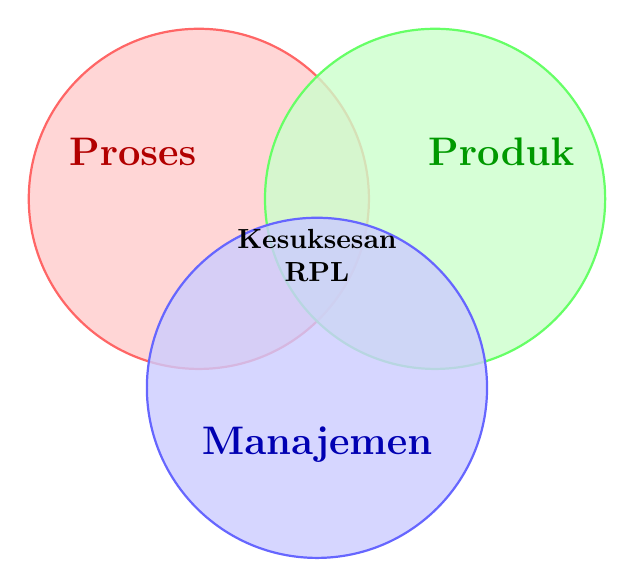
\begin{tikzpicture}[scale=1.2]
        % Circle 1: Proses
        \fill[red!20, opacity=0.8] (0, 1) circle (1.8);
        \draw[red!60, thick] (0, 1) circle (1.8);
        \node[text=red!70!black, font=\Large\bfseries] at (-0.7, 1.5) {Proses};

        % Circle 2: Produk
        \fill[green!20, opacity=0.8] (2.5, 1) circle (1.8);
        \draw[green!60, thick] (2.5, 1) circle (1.8);
        \node[text=green!60!black, font=\Large\bfseries] at (3.2, 1.5) {Produk};

        % Circle 3: Manajemen
        \fill[blue!20, opacity=0.8] (1.25, -1) circle (1.8);
        \draw[blue!60, thick] (1.25, -1) circle (1.8);
        \node[text=blue!70!black, font=\Large\bfseries] at (1.25, -1.6) {Manajemen};
        
        % Core intersection
        \node[font=\bfseries, align=center] at (1.25, 0.4) {Kesuksesan\\RPL};
    \end{tikzpicture}
    \caption{Tiga Pilar Utama Pembentuk Disiplin Rekayasa Perangkat Lunak.}
\end{figure}

\begin{enumerate}
    \item \textbf{Proses:} Mengacu pada langkah-langkah, metode, dan \textit{framework} (kerangka kerja) teknis yang digunakan untuk membangun sistem.
    \item \textbf{Produk:} Wujud nyata dari \textit{software} yang dihasilkan, baik itu kode, desain arsitektur, hingga dokumentasinya. Harus terukur kualitasnya.
    \item \textbf{Manajemen:} Urusan mengelola sumber daya manusia (tim), mengatur jadwal, mengatur biaya (\textit{budgeting}), dan memastikan risiko terkendali.
\end{enumerate}

\subsection{Proses Aktivitas Dasar Profesional}
Dalam pengembangan perangkat lunak secara profesional, ada empat aktivitas mendasar yang selalu dilakukan secara sekuensial atau iteratif:
\begin{enumerate}
    \item \textbf{Analisis (Spesifikasi):} Mencari tahu dan merumuskan apa yang sebenarnya dibutuhkan oleh pelanggan (\textit{requirements}).
    \item \textbf{Perancangan (Desain):} Menerjemahkan kebutuhan tadi menjadi cetak biru (\textit{blueprint}) arsitektur sistem, basis data, dan antarmuka.
    \item \textbf{Implementasi:} Menulis baris kode program (\textit{coding}) berdasarkan desain yang sudah dibuat.
    \item \textbf{Pengujian (\textit{Testing}):} Memastikan kode yang dibuat bebas dari *bug* dan benar-benar berjalan sesuai keinginan pelanggan.
\end{enumerate}

Selain aktivitas dasar di atas, pembelajaran RPL secara utuh akan mencakup berbagai topik spesifik seperti: Metode Pengembangan, Manajemen Proyek, Pembuatan Dokumen Spesifikasi, Pemodelan Diagram (UML: \textit{Use Case, Activity, Sequence, Class}), Perancangan Antarmuka (UI/UX), hingga Penjaminan Kualitas (QA).

\newpage
\section{Evolusi dan Jenis Aplikasi Perangkat Lunak}

Seiring berjalannya waktu, karakteristik perangkat lunak yang dikembangkan oleh manusia mengalami perubahan dan lompatan yang sangat drastis.

\subsection{Evolusi Perangkat Lunak}
Perkembangan historis \textit{software} dapat dibagi menjadi empat era besar:

\begin{table}[h]
\centering
\begin{tabular}{@{}p{3cm}p{11cm}@{}}
\toprule
\textbf{Timeline Era} & \textbf{Karakteristik Utama} \\ \midrule
\textbf{Era 1} \newline (1950 - 1960) & \textit{Beberapa Tahun Lalu.} Perangkat lunak murni berorientasi \textit{batch} (diproses berbarengan di akhir). Distribusinya sangat terbatas dan hanya dibuat kustom (\textit{custom software}) untuk perusahaan tertentu saja. \\ \addlinespace
\textbf{Era 2} \newline (1960 - 1970) & Sudah mulai mendudung fitur \textit{Multiuser} dan bekerja secara seketika (\textit{Real-time}). Di era ini pula konsep Basis Data (\textit{Database}) mulai muncul, serta software mulai dijual sebagai produk kemasan (\textit{Product software}). \\ \addlinespace
\textbf{Era 3} \newline (1970 - 1990) & Masuk ke fase sistem terdistribusi. Munculnya kecerdasan yang ditanamkan (\textit{Embedded "intelligence"}) pada perangkat keras berbiaya rendah. Perangkat lunak mulai memberi dampak masif bagi konsumen rumah tangga. \\ \addlinespace
\textbf{Era 4} \newline (1990 - 2000an)& Komputer meja (\textit{Desktop}) menjadi sangat canggih. Lahirnya teknologi berorientasi objek (\textit{Object-oriented technologies}), sistem pakar (\textit{Expert systems}), Jaringan Saraf Tiruan (AI), komputasi paralel, hingga sistem berbasis Jaringan/Internet. \\ \bottomrule
\end{tabular}
\caption{Garis Waktu Evolusi Perangkat Lunak.}
\end{table}

\subsection{Berbagai Kategori Aplikasi Perangkat Lunak}
Hari ini, perangkat lunak menopang hampir seluruh aspek kehidupan manusia. Berdasarkan fungsinya, \textit{software} bisa dikategorikan menjadi 9 jenis utama:
\begin{enumerate}
    \item \textbf{System Software:} Program yang melayani program lain (cth: Sistem Operasi seperti Windows, Linux).
    \item \textbf{Real-time Software:} Memonitor dan merespon peristiwa di dunia nyata seketika itu juga (cth: sistem navigasi pesawat).
    \item \textbf{Business Software:} Mengelola data bisnis dan operasional perusahaan (cth: sistem penggajian, \textit{point of sales}).
    \item \textbf{Engineering and Scientific Software:} Perhitungan kompleks untuk ilmuwan (cth: simulasi astronomi, CAD).
    \item \textbf{Embedded Software:} \textit{Software} yang ditanam ke dalam perangkat keras spesifik (cth: *software* di dalam mesin cuci atau \textit{microwave}).
    \item \textbf{Artificial Intelligence (AI) Software:} Memecahkan masalah rumit tanpa algoritma perhitungan pasti (cth: \textit{machine learning}, pengenalan suara).
    \item \textbf{Internet Software:} Aplikasi yang diakses melalui peramban web.
    \item \textbf{Software Tools and CASE environment:} \textit{Software} yang dipakai untuk membantu pemrogram membuat \textit{software} lain (cth: IDE, compiler).
    \item \textbf{Produk Developer:} Aplikasi generik (bisa dipakai siapa saja, cth: MS Word) atau aplikasi kustom (pesanan khusus satu perusahaan).
\end{enumerate}

\end{document}